\chapter{Appendix A}
\ifpdf
    \graphicspath{{Appendix1/images/}}
\else
    \graphicspath{{Appendix1/images/}}
\fi

\section{About the SR3 SSIM regularized model}

SR3 algorithm works very similar to the original DDPM paper \cite{ho2020denoising}. The training can be described as follows: \\

\begin{enumerate}
    \item repeat

    \item $(x, y_0)$ $\sim$ $p(x,y)$

    \item $\gamma$ $\sim$ p($\gamma$)

    \item $\epsilon$ $\sim$ \mathcal{N}(0, I)

    \item Take a gradient descent step on:
        
        $$ - (\nabla_{\theta}  NPSNR(f_{\theta}(x, y_{t}, \gamma_{t}), \epsilon) + \lambda * SSIM(f_{\theta}(x, y_{t}, \gamma_{t}), \epsilon))$$

    \item until converged
    
\end{enumerate}

\nomenclature[znpsnr]{$NPSNR$}{Normalized Peak Signal-to-Noise Ratio}
\nomenclature[gn]{$\nabla$}{Gradient of a function}
\nomenclature[gg]{$\gamma$}{The variance schedule}
\nomenclature[s0]{$t$}{timestep t}

The above describes the training process, where a random sample is picked, x is the bicubic interpolated image from the LR image and $y_{0}$ is the HR image, $\gamma_{t}$ is the variance schedule constant and it is assumed to be a constant in the model for a given t.\\

The model is used to obtain the SR image back using a T step refinement process as described below in the original SR3 paper.

\begin{figure}[!htbp]
  \begin{center}
    \leavevmode
    \ifpdf
      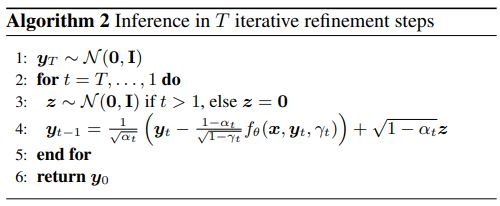
\includegraphics[height=2in]{Appendix1/images/WhatsApp Image 2023-05-08 at 17.34.05.jpg}
    \else
      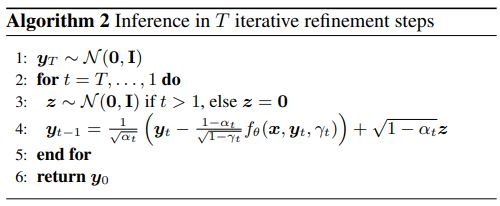
\includegraphics[bb = 50 86 545 742, height=6in]{Appendix1/images/WhatsApp Image 2023-05-08 at 17.34.05.jpg}
    \fi
    \caption{Inference process in T steps using the model learnt in training \cite{saharia2021image}}
    \label{inference_sr3}
  \end{center}
\end{figure}

\begin{figure}[!htbp]
  \begin{center}
    \leavevmode
    \ifpdf
      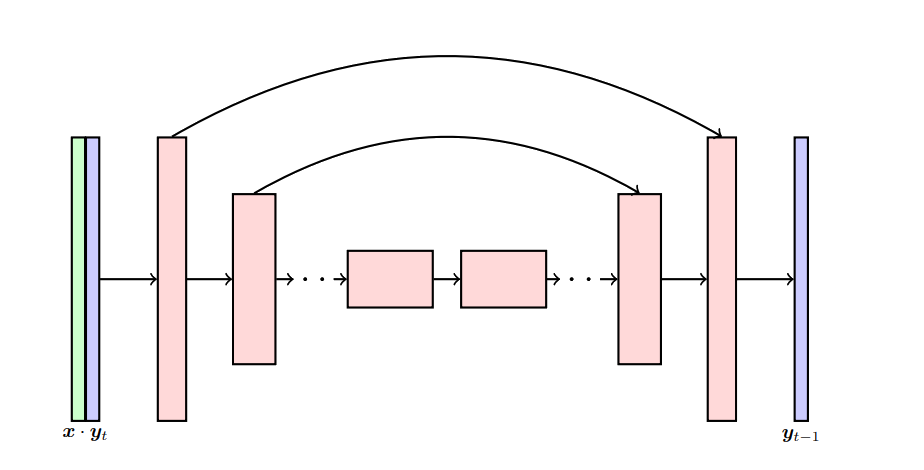
\includegraphics[height=3in]{Appendix1/images/sr3-new.png}
    \else
      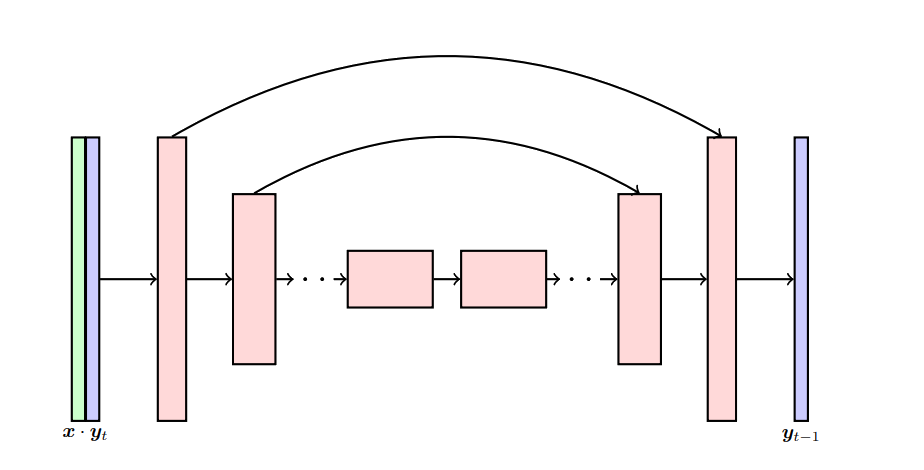
\includegraphics[bb = 92 86 545 742, height=6in]{Appendix1/images/sr3-new.png}
    \fi
    \caption{ Outline of the U-Net showing the input x (the bicubic interpolated image), $y_t$ (the noisy image at timestep t) and the output as $y_{t-1}$ obtained using Algorithm 2 (the noisy image at timestep t-1, less noisy than at timestep t) \cite{saharia2021image}}
    \label{u_net_sr3}
  \end{center}
\end{figure}

\section{Architecture details of our model}

We have trained a variation of the SR3 i.e., SSIM regularized SR3 network with the following details.

\begin{enumerate}
    \item We have focused on the task of converting 64 X 64 MR images to 512 X 512 image datasets.
    \item We have used a pre-trained model (taken from \underline{\href{https://github.com/Janspiry/Image-Super-Resolution-via-Iterative-Refinement}{Janspiry's GitHub page}}), trained on human faces using FFHQ-CelebaHQ dataset \cite{karras2018progressive, karras2019stylebased}.
    \item Other details are included in the table below

    \vspace*{0.3cm}
    \begin{table}[h]
    \begin{center}
    \begin{tabular}{ p{6cm} m{6cm}}
     \hline
     \multicolumn{2}{c}{} \\
     \hline
     \textbf{Channel Multipliers}    & \{1,2,4,8,16\} \\
     \textbf{Timestep T}& 2000\\
     \textbf{Variance Schedule}& Cosine Variance Schedule\\
     \textbf{Batch Size}& 1 (Low GPU memory)\\
     \textbf{Res Blocks}& 1\\
     \textbf{Dropout}& 0\\
     \textbf{Model Parameters}& 155M\\
     \textbf{Train steps}& 100K\\
     \hline
    \end{tabular}
    \end{center}
    \caption{Architecture Details of the Model}
    \label{W-Net table}
    \end{table}
    
\end{enumerate}

The FID model follows the same pattern as SSIM except for the function SSIM being replaced by FID and the architecture details also follow similarly to SSIM. The simple SR3 model also follows the same architecture and parameters but with the absence of regularization.

% ------------------------------------------------------------------------

%%% Local Variables: 
%%% mode: latex
%%% TeX-master: "../thesis"
%%% End: 
